\chapter{Interval graphs}

An interval graph is a graph $G$ that is the intersection graph of a collection
of closed intervals in $\mathbb{R}$.

First we present the main characterizations of interval graphs. In the next sections we present some other subclasses of interval graphs that will help us characterize the thin strip graphs on chapter \ref{chap:thinDef}.

\section{Interval graphs}
Interval graphs

\begin{theorem}[Fishburn \cite{FISHBURN1985135}]
  \label{theo:intervalChord}
  $G$ is an interval graph if and only if every simple cycle of four or more
  points has a chord and any three independent vertices can be ordered ($u<v<w$) such that every path from $u$ to $w$ passes through a neighbour of $v$.
\end{theorem}



\section{Unit interval graphs}

If the length of each interval is unitary,
then $G$ is a unit interval graph (UIG). UIG is equivalent to the proper interval graphs class, where no interval can be properly included in another one
\cite{roberts1968representations}.

\begin{theorem}[Roberts \cite{roberts1968representations}]
  An interval graph is a unit interval graph if and only if it has no induced subgraph $K_{1,3}$.
\end{theorem}

\section{Mixed unit interval graphs}
\label{sec:muig}

Another interesting class of interval graphs are mixed unit interval graphs, where each
interval is unitary and can be closed, open, open-closed or closed-open. In this paper we will
denote those four classes like this:

$$\mathcal{I}^{++} = \{[x,y] : x,y \in \mathbb{R}, x\leq y\}$$
$$\mathcal{I}^{--} = \{(x,y) : x,y \in \mathbb{R}, x\leq y\}$$
$$\mathcal{I}^{+-} = \{[x,y) : x,y \in \mathbb{R}, x\leq y\}$$
$$\mathcal{I}^{-+} = \{(x,y] : x,y \in \mathbb{R}, x\leq y\}$$

$\mathcal{I}$ will be replaced by $\mathcal{U}$ when we are talking about unit
mixed interval graphs and their class is denoted MUIG.

\begin{theorem}
  The classes of the graphs $\mathcal{U}^{--}$, $\mathcal{U}^{++}$,
  $\mathcal{U}^{-+}$, $\mathcal{U}^{+-}$, and  $\mathcal{U}^{-+} \cup
  \mathcal{U}^{+-}$ are the same (equivalent for $\mathcal{I}$). \cite{DOURADO20123357}
\end{theorem}

\begin{figure}
\centering
\begin{scaletikzpicturetowidth}{\textwidth}
\begin{tikzpicture}[scale=1.5]

  \draw[{(-)}] (-1,-0.5) -- (0,-0.5);
  \draw[color=black] (-0.4845,-0.8507) node {$v_4$};
  \draw[{[-}] (0,-1.5) -- (1,-1.5);
  \draw[color=black] (0.5023,-1.3568) node {$v_3$};
  \draw[{-]}] (-2,-1.5) -- (-1,-1.5);
  \draw[color=black] (-0.4899,-0.3468) node {$v_2$};
  \draw[{[-]}] (-1,-1) -- (0,-1);
  \draw[color=black] (-1.4962,-1.3536) node {$v_1$};

  \node[draw,circle,inner sep=2pt,fill,label distance=1cm] (v1) at (-4,-0.25) {};
  \draw[color=black] (-4,0) node {$v_4$};
  \node[draw,circle,inner sep=2pt,fill,label distance=1cm] (v3) at (-4,-1.25) {};
  \draw[color=black] (-4,-1.5) node {$v_2$};
  \node[draw,circle,inner sep=2pt,fill,label distance=1cm] (v2) at (-5,-1.25) {};
  \draw[color=black] (-3,-1.5) node {$v_3$};
  \node[draw,circle,inner sep=2pt,fill,label distance=1cm] (v4) at (-3,-1.25) {};
  \draw[color=black] (-5,-1.5) node {$v_1$};
  \draw  (v1) edge (v2);
  \draw  (v1) edge (v3);
  \draw  (v1) edge (v4);

\end{tikzpicture}
\end{scaletikzpicturetowidth}

\caption{Representation of $K_{1,3}$ as a MUIG.}
\label{fig:muigK13}
\end{figure}

Unlike for UIG class, $K_{1,3}$ is a MUIG as seen in figure \ref{fig:muigK13}. A complete characterization by induced forbidden subgraphs have been found independently by F. Joos \cite{shuchatUnitMixedInterval2014a} and A. Schuchat et al. \cite{joosCharacterizationMixedUnit2013}. In the next subsection the characterization of F. Joos will be reviewed by adding some remarks about graph inclusions.

\subsection{Characterization}

Joos proves in his paper the following theorem:

\begin{theorem}[Joos \cite{joosCharacterizationMixedUnit2013}]
  $G$ is a MUIG if and only if it is a $\{F\}\cup\mathcal{R}\cup\mathcal{S}\cup\mathcal{S''}\cup\mathcal{T}$-free interval graph.
\end{theorem}

We will present each family of forbidden induced subgraphs and analyze whether they are included in other relevant classes of graphs (e.g. unit disk graphs). Only properties that will be used in next chapters will be presented,

\begin{figure}
\begin{center}
  \begin{scaletikzpicturetowidth}{\textwidth}
  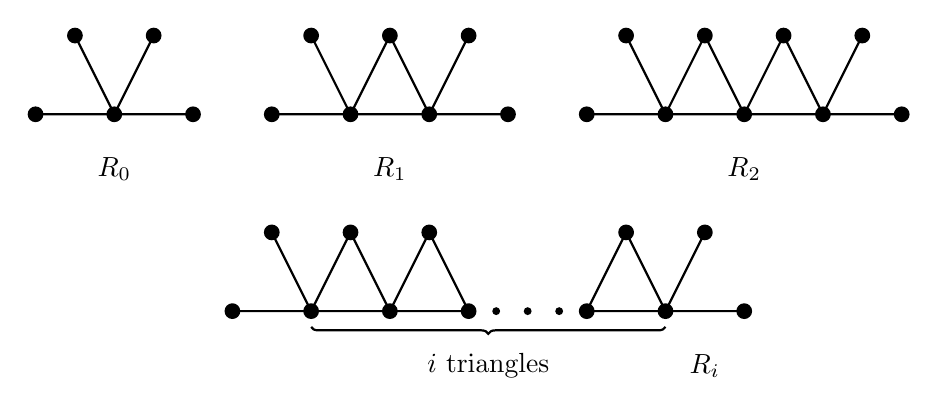
\begin{tikzpicture}[scale=1]
\def\ver{0.1} %size of a vertex
\def\x{1}

\def\xa{0.5}
\def\ya{0}

\def\xb{4}
\def\yb{0}

\def\xc{8}
\def\yc{0}

\def\xd{3.5}
\def\yd{-2.5}


%graph R_0
\path[fill] (\xa+0.5,\ya) circle (\ver);
\path[fill] (\xa+1,\ya+1) circle (\ver);
\path[fill] (\xa+2,\ya+1) circle (\ver);
\path[fill] (\xa+2.5,\ya) circle (\ver);
\path[fill] (\xa+1.5,\ya) circle (\ver);

\draw[thick] (\xa+0.5,\ya)--(\xa+1.5,\ya)--(\xa+1,\ya+1)
(\xa+2,\ya+1)--(\xa+1.5,\ya)--(\xa+2.5,\ya);

\node (1) at (\xa+1.5,\ya-0.7) {$R_0$};

%graph R_1
\path[fill] (\xb,\yb) circle (\ver);
\path[fill] (\xb+1,\yb) circle (\ver);
\path[fill] (\xb+2,\yb) circle (\ver);
\path[fill] (\xb+3,\yb) circle (\ver);
\path[fill] (\xb+0.5,\yb+1) circle (\ver);
\path[fill] (\xb+1.5,\yb+1) circle (\ver);
\path[fill] (\xb+2.5,\yb+1) circle (\ver);

\draw[thick] (\xb,\yb)--(\xb+1,\yb)--(\xb+2,\yb)--(\xb+3,\yb)
(\xb+0.5,\yb+1)--(\xb+1,\yb)--(\xb+1.5,\yb+1)--(\xb+2,\yb)--(\xb+2.5,\yb+1);

\node (1) at (\xb+1.5,\yb-0.7) {$R_1$};


%graph R_2
\path[fill] (\xc,\yc) circle (\ver);
\path[fill] (\xc+1,\yc) circle (\ver);
\path[fill] (\xc+2,\yc) circle (\ver);
\path[fill] (\xc+3,\yc) circle (\ver);
\path[fill] (\xc+4,\yc) circle (\ver);
\path[fill] (\xc+0.5,\yc+1) circle (\ver);
\path[fill] (\xc+1.5,\yc+1) circle (\ver);
\path[fill] (\xc+2.5,\yc+1) circle (\ver);
\path[fill] (\xc+3.5,\yc+1) circle (\ver);

\draw[thick] (\xc,\yc)--(\xc+1,\yc)--(\xc+2,\yc)--(\xc+3,\yc)--(\xc+4,\yc)
(\xc+0.5,\yc+1)--(\xc+1,\yc)--(\xc+1.5,\yc+1)--(\xc+2,\yc)--(\xc+2.5,\yc+1)--(\xc+3,\yc)--(\xc+3.5,\yc+1);

\node (1) at (\xc+2,\yc-0.7) {$R_2$};

%graph R_i
\path[fill] (\xd,\yd) circle (\ver);
\path[fill] (\xd+1,\yd) circle (\ver);
\path[fill] (\xd+2,\yd) circle (\ver);
\path[fill] (\xd+3,\yd) circle (\ver);
\path[fill] (\xd+4.5,\yd) circle (\ver);
\path[fill] (\xd+5.5,\yd) circle (\ver);
\path[fill] (\xd+6.5,\yd) circle (\ver);
\path[fill] (\xd+0.5,\yd+1) circle (\ver);
\path[fill] (\xd+1.5,\yd+1) circle (\ver);
\path[fill] (\xd+2.5,\yd+1) circle (\ver);
\path[fill] (\xd+5,\yd+1) circle (\ver);
\path[fill] (\xd+6,\yd+1) circle (\ver);

\fill (\xd+3.35,\yd) circle (\ver/2);
\fill (\xd+3.75,\yd) circle (\ver/2);
\fill (\xd+4.15,\yd) circle (\ver/2);

\draw[thick] (\xd,\yd)--(\xd+3,\yd)
(\xd+4.5,\yd)--(\xd+6.5,\yd)
(\xd+0.5,\yd+1)--(\xd+1,\yd)--(\xd+1.5,\yd+1)--(\xd+2,\yd)--(\xd+2.5,\yd+1)--(\xd+3,\yd)
(\xd+4.5,\yd)--(\xd+5,\yd+1)--(\xd+5.5,\yd)--(\xd+6,\yd+1);

\draw[thick,decoration={brace,mirror,raise=0.2cm},decorate] (\xd+1,\yd) -- (\xd+5.5,\yd)
node [pos=0.5,anchor=north,yshift=-0.4cm] {$i$ triangles};

\node (1) at (\xd+6,\yd-0.7) {$R_i$};

\end{tikzpicture}
\end{scaletikzpicturetowidth}
\end{center}
\caption{The class $\mathcal{R}$. \cite{joosCharacterizationMixedUnit2013}}\label{graphsR}
\end{figure}



\begin{figure}[t]
\begin{center}
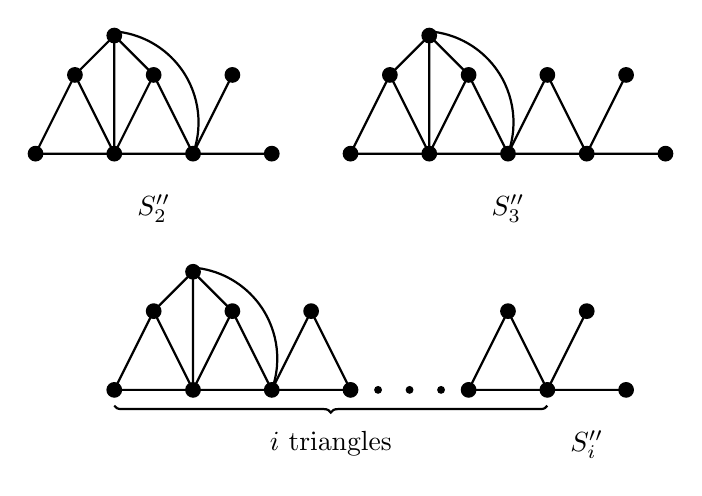
\begin{tikzpicture}[scale=1]
\def\ver{0.1} %size of a vertex
\def\x{1}

\def\xa{2}
\def\ya{-3}

\def\xb{0}
\def\yb{0}

\def\xc{0}
\def\yc{0}

\def\xd{5}
\def\yd{0}

%graph S^2_2
\path[fill] (\xc,\yc) circle (\ver);
\path[fill] (\xc+1,\yc) circle (\ver);
\path[fill] (\xc+2,\yc) circle (\ver);
\path[fill] (\xc+3,\yc) circle (\ver);
\path[fill] (\xc+0.5,\yc+1) circle (\ver);
\path[fill] (\xc+1.5,\yc+1) circle (\ver);
\path[fill] (\xc+2.5,\yc+1) circle (\ver);
\path[fill] (\xc+1,\yc+1.5) circle (\ver);


\draw[thick] (\xc,\yc)--(\xc+1,\yc)--(\xc+2,\yc)--(\xc+3,\yc)
(\xc+0.5,\yc+1)--(\xc+1,\yc)--(\xc+1.5,\yc+1)--(\xc+2,\yc)--(\xc+2.5,\yc+1)
(\xc,\yc)--(\xc+0.5,\yc+1)--(\xc+1,\yc+1.5)--(\xc+1.5,\yc+1)
(\xc+1,\yc)--(\xc+1,\yc+1.5);

\draw[thick] (\xc+2,\yc) arc(-20:85:1.16);

\node (1) at (\xc+1.5,\yc-0.7) {$S_2''$};

%graph S^2_3
\path[fill] (\xd-1,\yd) circle (\ver);
\path[fill] (\xd-0.5,\yd+1) circle (\ver);
\path[fill] (\xd,\yd) circle (\ver);
\path[fill] (\xd+1,\yd) circle (\ver);
\path[fill] (\xd+2,\yd) circle (\ver);
\path[fill] (\xd+3,\yd) circle (\ver);
\path[fill] (\xd+0.5,\yd+1) circle (\ver);
\path[fill] (\xd+1.5,\yd+1) circle (\ver);
\path[fill] (\xd+2.5,\yd+1) circle (\ver);
\path[fill] (\xd,\yd+1.5) circle (\ver);


\draw[thick] (\xd-1,\yd)--(\xd+3,\yd)
(\xd-1,\yd)--(\xd-0.5,\yd+1)--(\xd,\yd)--(\xd+0.5,\yd+1)--(\xd+1,\yd)--(\xd+1.5,\yd+1)--(\xd+2,\yd)--(\xd+2.5,\yd+1)
(\xd-0.5,\yd+1)--(\xd,\yd+1.5)--(\xd+0.5,\yd+1)
(\xd,\yd)--(\xd,\yd+1.5);

\draw[thick] (\xd+1,\yd) arc(-20:85:1.16);

\node (1) at (\xd+1,\yd-0.7) {$S_3''$};

%graph S_i''
\path[fill] (\xa-1,\ya) circle (\ver);
\path[fill] (\xa,\ya) circle (\ver);
\path[fill] (\xa+1,\ya) circle (\ver);
\path[fill] (\xa+2,\ya) circle (\ver);
\path[fill] (\xa+3.5,\ya) circle (\ver);
\path[fill] (\xa+4.5,\ya) circle (\ver);
\path[fill] (\xa+5.5,\ya) circle (\ver);
\path[fill] (\xa-0.5,\ya+1) circle (\ver);
\path[fill] (\xa+0.5,\ya+1) circle (\ver);
\path[fill] (\xa+1.5,\ya+1) circle (\ver);
\path[fill] (\xa+4,\ya+1) circle (\ver);
\path[fill] (\xa+5,\ya+1) circle (\ver);
\path[fill] (\xa,\ya+1.5) circle (\ver);


\draw[thick] (\xa-1,\ya)--(\xa+2,\ya)
(\xa+3.5,\ya)--(\xa+5.5,\ya)
(\xa-1,\ya)--(\xa-0.5,\ya+1)--(\xa,\ya)--(\xa+0.5,\ya+1)--(\xa+1,\ya)--(\xa+1.5,\ya+1)--(\xa+2,\ya)
(\xa+3.5,\ya)--(\xa+4,\ya+1)--(\xa+4.5,\ya)--(\xa+5,\ya+1)
(\xa-0.5,\ya+1)--(\xa,\ya+1.5)--(\xa+0.5,\ya+1)
(\xa,\ya)--(\xa,\ya+1.5);

\draw[thick] (\xa+1,\ya) arc(-20:85:1.16);

\node (1) at (\xa+5,\ya-0.7) {$S_i''$};

\fill (\xa+2.35,\ya) circle (\ver/2);
\fill (\xa+2.75,\ya) circle (\ver/2);
\fill (\xa+3.15,\ya) circle (\ver/2);

\draw[thick,decoration={brace,mirror,raise=0.2cm},decorate] (\xa-1,\ya) -- (\xa+4.5,\ya)
node [pos=0.5,anchor=north,yshift=-0.4cm] {$i$ triangles};


\end{tikzpicture}
\end{center}
\caption{The class $\mathcal{S}''$.}\label{graphsSS}
\end{figure}


\lemma{$\mathcal{R}$ is a family of co-comparability graphs.}
\proof{If we recall Theorem \ref{theo:spanning}, in order to prove that $\mathcal{R}$ is a family of co-comparability graphs we will have to find a spanning order for every $R_i$ with $i \geq 0$. We will proceed to label our vertices with a mapping function $f: V \to \mathbb{N}$ such that $f(v) \in [1,|V|]$. This mapping will give us a spanning order by induction:

\begin{itemize}
  \item $i = 0$: We assign the number $1$ to the vertex with maximum degree $v_1$. We assign then the rest of the numbers to the other vertices. We see then that $\forall u < v < w : uw\in E \to uv \in E$ because every vertex is adjacent to $v_1$.

  \item $i = i+1$: We define $\lambda_i = 5+2i$ where $\lambda_i = |V(R_i)|$. We have two on each graph, where their labels are $\lambda_i+1$ and $\lambda_i+2$ and there are three new edges: $v_{\lambda_i}v_{\lambda_i-1},v_{\lambda_i}v_{\lambda_i+1},v_{\lambda_i}v_{\lambda_i+2} \in E$.

  By induction we only have to see if it holds with the new edges. We can say that it still holds with $v_{\lambda_i}v_{\lambda_i-1}$ and $v_{\lambda_i}v_{\lambda_i+1}$ because:

  $$\nexists k \in \mathbb{N} : i < k < i+1$$

  Finally, we see that $v_{\lambda_i}v_{\lambda_i+2}$ is a valid edge because $v_{\lambda_i}v_{\lambda_i+1}\in E$. \qed
\end{itemize}
}

\begin{figure}
\begin{center}
  \begin{scaletikzpicturetowidth}{\textwidth}
  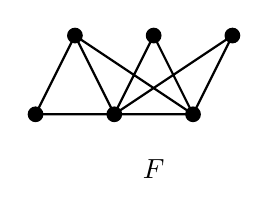
\begin{tikzpicture}[scale=1]
    \def\ver{0.1} %size of a vertex
    \def\x{1}

    \def\xa{0}
    \def\ya{0}

    %G_1
    \path[fill] (\xa+1,\ya) circle (\ver);
    \path[fill] (\xa+2,\ya) circle (\ver);
    \path[fill] (\xa+0.5,\ya+1) circle (\ver);
    \path[fill] (\xa+1.5,\ya+1) circle (\ver);
    \path[fill] (\xa+2.5,\ya+1) circle (\ver);
    \fill (\xa,\ya) circle (\ver);

    \draw[thick] (\xa+1,\ya)--(\xa+2,\ya)
    (\xa+1,\ya)--(\xa+0.5,\ya+1)--(\xa+2,\ya)
    (\xa+1,\ya)--(\xa+2.5,\ya+1)--(\xa+2,\ya)
    (\xa+1,\ya)--(\xa+1.5,\ya+1)--(\xa+2,\ya)
    (\xa+1,\ya)--(\xa,\ya)--(\xa+0.5,\ya+1);

    \node (1) at (\xa+1.5,\ya-0.7) {$F$};

\end{tikzpicture}
\end{scaletikzpicturetowidth}
\end{center}
\caption{The graph $F$. \cite{joosCharacterizationMixedUnit2013}}\label{graphG1}
\end{figure}

\section{Unfettered unit interval graphs}
\label{sec:UUIG}

An unfettered unit interval graph can be defined as an interval graph such that for every touching

Hayashi has characterized this class of graphs by levels. A \textit{level structure} of a graph $G = (V,E)$ is a partition $L = \{L_i : i \in [1,t]\}$ of $V$ such that

$$v \in L_k \to N(v) \subseteq L_{k-1} \cup L_{k} \cup L_{k+1}$$

where $L_0 = L_t+1 = \varnothing$.

\begin{theorem}[Hayashi et al. \cite{hayashiThinStripGraphs2017}]
  \label{theo:uuig_char}
  A graph $G$ is an unfettered unit interval graph if and only if it has a level structure where each level is a clique.
\end{theorem}

We can clearly see that MUIG $\in$ UUIG. However, we still have to see what is the location of UUIG in the higher graph classes hierarchy:

\begin{prop}
  UUIG $\subset$ co-comparability.
\end{prop}

\proof{For each vertex of a partition $L_k$ of UUIG (Theorem \ref{theo:uuig_char}) we assign arbitrarily a number $i \in [\max(V(L_{k-1}))+1,\max(V(L_{k-1}))+|V(L_k)|+1]$; intuitively, we assign every available number from the beginning in order ($|V(L_1)|$ first numbers on the first partition and consecutively).

Because we know that each partition $L_k$ is a clique, we can say that for each three vertices $u < v < w$, if $vw \in E \to uv\in E\  \text{or} \ vw\in E$. We know this because given $u \in L_i$ and $w \in L_j$: if $uw\in E$ it means that levels $L_i$ and $L_j$ are adjacent, which means that $v\in L_i$ or $v\in L_j$ so $v$ will be adjacent either to $u$ or $w$. \qed
}
